\documentclass[conference]{IEEEtran}
\IEEEoverridecommandlockouts
% The preceding line is only needed to identify funding in the first footnote. If that is unneeded, please comment it out.

\usepackage[acronym]{glossaries}
\usepackage{cite}
\usepackage{amsmath,amssymb,amsfonts}
\usepackage{algorithmic}
\usepackage{graphicx}
\usepackage{textcomp}
\usepackage{xcolor}

\usepackage{listings}
% \usepackage{biblatex}
\usepackage{adjustbox}
\usepackage{tabulary}

\usepackage{todonotes}
\newcommand{\db}[1]{\textcolor{blue!40}{#1}}
\newcommand{\dbc}[1]{\todo[author=Dilum, inline, color=blue!40]{#1}}
\newcommand{\gk}[1]{\textcolor{green!50}{#1}}
\newcommand{\gkc}[1]{\todo[author=Gihan, inline, color=green!50]{#1}}

\usepackage{hyperref}
\usepackage{cleveref}

\crefformat{section}{#2Sec.~#1#3}
\crefformat{figure}{#2Fig.~#1#3}

% \addbibresource{mendeley.bib}

\definecolor{codegreen}{rgb}{0,0.6,0}
\definecolor{backcolour}{rgb}{0.95,0.95,0.92}
\lstdefinestyle{code-style}{
  backgroundcolor=\color{backcolour}, commentstyle=\color{codegreen},
  basicstyle=\ttfamily\footnotesize,
  breakatwhitespace=false,
  breaklines=true,
  captionpos=b,
  keepspaces=true,
  numbers=left,
  numbersep=5pt,
  showspaces=false,
  showstringspaces=false,
  showtabs=false,
  tabsize=2
}
\lstset{style=code-style}

\def\BibTeX{{\rm B\kern-.05em{\sc i\kern-.025em b}\kern-.08em
    T\kern-.1667em\lower.7ex\hbox{E}\kern-.125emX}}
    
\begin{document}

\title{WDIAS: A Microservices-Based Weather Data Integration and Assimilation System\\
}

\author{\IEEEauthorblockN{Gihan Karunarathne}
\IEEEauthorblockA{\textit{Dept. Computer Science and Engineering} \\
\textit{University of Moratuwa}\\
Katubedda, Sri Lanka \\
gihan.09@cse.mrt.ac.lk}
\and
\IEEEauthorblockN{H.M.N. Dilum Bandara}
\IEEEauthorblockA{\textit{Dept. Computer Science and Engineering} \\
\textit{University of Moratuwa}\\
Katubedda, Sri Lanka \\
dilumb@cse.mrt.ac.lk}
\and
\IEEEauthorblockN{Srikantha Herath}
\IEEEauthorblockA{\textit{Center for Urban Water, Sri Lanka} \\
Battaramulla, Sri Lanka \\
admin@curwsl.org}
}

\maketitle

%%%%%%%%%%%%%%%%%%%%%%%%%%%%%%%%%%%%%%%%%%%%%%%%%%%%%%%%%%%%%%%%%%%%%%%%%%%%%%%%
\begin{abstract}
Numerical Weather Models (NWMs) utilize data from diverse sources such as automated weather stations, radars, and satellite images. Such multimodal data need to be transcoded into a NWM compatible format before use. Moreover, the data integration system's response time needs to be relatively low to reduce the time to forecast weather events like hurricanes and flash floods. Furthermore, the resulting data need to be accessed by many researchers and third-party applications. Existing weather data integration systems are based on monolithic or client-server architectures, and are proprietary or closed source. Hence, they are not only expensive to operate in an era of cloud computing, but also challenging to customize for regions with different weather patterns. In this paper, we present a Weather Data Integration and Assimilation System (WDIAS) that uses microservices architecture and container orchestration to achieve high scalability, availability, and low-cost operation. WDIAS provides a modular architecture to integrate data from different sources, enforce data quality controls, export data into different formats, and extend the functionality by adding new modules. Using a synthetic workload and an experimental setup on a public cloud, we demonstrate that WDIAS can handle 300 requests per second with relatively low latency.
\end{abstract}


\begin{IEEEkeywords}
Cloud computing, data assimilation, data integration, microservice, weather
\end{IEEEkeywords}

%%%%%%%%%%%%%%%%%%%%%%%%%%%%%%%%%%%%%%%%%%%%%%%%%%%%%%%%%%%%%%%%%%%%%%%%%%%%%%%%
\section{Introduction}
\label{pse:Introduction}
%Weather prediction is essential to reduce the impacts caused by natural disasters and to effectively manage natural water resources. To enhance the accuracy of weather predictions, it requires to provide reliable and detailed weather data as inputs to \acrfull{nwm}s. Before feeding such diverse data collected from different sources, we need to convert data into NWMs compatible data format. Further we need to process data with lesser time to increase the lead time of forecasting, and need to handle bulk stream weather data.
%Many third-party applications and researcher need to accessed processed weather data to make use of them. As few examples, logistics companies could use those data with their models to plan and schedule their deliveries. Agricultural insurance companies can warn the farmers, as well as calculate premiums based on anticipated weather patterns.
%Even though there are many data integration systems, most systems are proprietary or closed source. For an island like Sri Lanka that having different kinds of weather seasons over the year than that software originated countries, those systems need to be highly customized. Thus it required to get support from the vendor to integrate and configure the system.
%Most of the software existing out there are not up to date with the latest technology concepts such as Cloud Computing, and not using modern architecture pattern like microservice architecture that can use to build highly scalable and available systems, and use containerized applications to run systems independ of software platforms.

Weather prediction is essential to reduce impact due to natural disasters and to manage natural resources like water effectively. To enhance the accuracy of weather predictions, it is necessary to provide reliable and detailed weather data as inputs to \acrfull{nwm}s. Before feeding multimodal data collected from different sources into a NWM, they need to be converted to a format that can be ingested by the NWM. Further, the velocity and volume of data vary from event-driven bulk uploads to streaming data. Such data need to be ingested, converted, stored, and accessed with minimal latency, especially when forecasting time-sensitive weather events. Processed weather data may also need to be accessed by many third-party applications and researchers. For example, logistics and insurance companies could use weather data for planning purposes or set their service fees or premiums based on anticipated weather patterns.

Several data integration systems are designed for weather-related use cases. For example, \acrshort{fews} \cite{Werner2013TheSystem} uses a model-centric approach where it handles the forecasting process as a combination of data modeling steps and data transformation algorithms. It creates forecasting workflows by integrating new models and algorithms based on the open model integration framework \cite{Kokkonen2003InterfacingXML}. \acrshort{fews} follows a common data model and enforces data access via a well-defined interface. While such a design leads to efficient data access and management, it requires all NWMs and connected systems to comply with the common data model, tightly couples the models, and serializes the model execution. 
\acrfull{lead} \cite{Droegemeier2005Service-OrientedWeather} provides dynamic workflow orchestration and data management based on Web-services. It provides several service layers based on the \acrfull{soa}, exposes services via a drag-and-drop interface to create new workflows, and aggregates computing resources into a pool. This design design results in a high performing, customizable, scalable, and resource-efficient weather analysis framework. 
\acrfull{dias} \cite{Kawasaki2018DataReduction} is another related system that provides efficient data storage, data quality controls, metadata management, and data sharing. \acrfull{madis} \cite{Macdermaid2005ArchitectureP2.39} enforces a common data format and provides role-based data access. 
However, \acrshort{dias} and \acrshort{madis} do not support workflows. All these systems are based on monolithic or client-service architectures and are platform dependent. Thus, they cannot gain the performance and economic benefits of contemporary technologies such as cloud computing. Further, these systems are either proprietary or closed source, limiting the wider adoption and customization. For example, it is challenging to customize them for an island like Sri Lanka with different weather patterns.

%, they are based on monolithic or client-server architectures. , mare not up to date with the latest technology concepts such as Cloud Computing, not using modern architecture pattern such as microservice architecture was able to provide high scalability and availability, and depend on the software platforms. most of them are proprietary or closed source. For an island like Sri Lanka that having different kinds of weather seasons over the year than that software originated need to be highly customized. Thus it required to get support from the vendor to integrate and configure the system.

% \db{Several forecasting systems are} developed with considering above factors for disaster management. Deltares developed the The \acrfull{fews}\cite{Werner2013TheSystem} in the Netherland for operational forecasting. It uses a model-centric approach, and implements the forecasting process as a combination of data modeling steps and data transformation algorithms. This framework does not have inherent hydrological modeling capabilities. But it capable of providing capability to create forecast workflows by integrate new models and algorithms. Also it uses a common data-model approach, and only allows models to interact with the system data via using one of the interfaces provided. All the timeseries data store in the common data model. This approach can consider as efficient for data store and access, but it has the inherent performance issues of access data in the database through a single data model. Interestingly, the \acrshort{fews} uses set of unique fields to identify timeseries one from another such as using timeseries's location and data type, as well as an id related to the source of the data. It provides an easy model integration with using the concept of the open modeling framework proposed by Open model integration \cite{Kokkonen2003InterfacingXML}. But the model adapter causes tide couple between models and the execution process of the \acrshort{fews}. This can cause issues when it required to do model unit testing and restrict the flexibility of running the models with parallel execution or external process execution.

% \acrfull{lead} \cite{Droegemeier2005Service-OrientedWeather} uses the concept of dynamic workflow orchestration and data management in a Web services framework. To predict and analyze weather models by researchers, it requires many resources. Rather than each researcher runs and maintain own computer resources for the weather experiments, the \acrshort{lead} provides a pool of resources. The researchers use the resources pool to run their experiment in shorter amounts of time in higher scale. The \acrshort{lead} follows \acrfull{soa} with different service layers. Also it exposes services through a drag and drop interface to create new workflows. A workflow service in the \acrshort{lead} schedules and run built workflows with promising the maximum use of underline resource pool. \acrfull{dias} \cite{Kawasaki2018DataReduction} and \acrfull{madis} \cite{Macdermaid2005ArchitectureP2.39} provide the functionality of integration and sharing weather data. When compared to other discussed systems, \acrshort{dias} and \acrshort{madis} do not provide the workflow capabilities. The \acrshort{dias} converts data using a inbuilt set of \acrshort{api}s to store data on a large volume of disk space. It also provides some functionalities to quality control the data, and metadata management, and shares the data through a shared API layer. The \acrshort{madis} stores the data after converts into a common data format, and allow role based data access.
% As mentioned above, most systems uses monolithic architecture or client service architecture, platform dependent, and not up to date with cloud computing technologies. Thus users can not benefit from modern cloud platforms and not able to decide the best cost-effective way to host the system. Since most systems are proprietary or closed source, it is difficult to add new requirements and maintain the system in long-term.

In this paper, we present a cloud-based \acrfull{wdias} that supports data integration, assimilation, and dissemination. We designed the proposed system based on the microservices architecture to make it highly scalable, available, modular, and extensible compared to related systems. \acrshort{wdias} can integrate both bulk and timeseries data from different sources, export data into different formats, and add extension modules for custom data transformations and quality controls. The proposed platform further uses container orchestration to simplify application management and gain cost savings through efficient use of cloud computing resources. 
Using an experimental setup on the cloud and synthetic workload derived from weather use cases, we demonstrate that \acrshort{wdias} can handle 300 requests (with different data types) per second. Also, the system is capable of running on a large range of computing resources ranging from a few CPUs to hundreds of CPUs, as well as show good elasticity against varying workloads.

The rest of the paper is organized as follows: The architecture of \acrshort{wdias} is presented in \cref{pse:wdias_architecture}. In \cref{pse:performance_analysis} we present the performance analysis. Concluding remarks are presented in \cref{pse:summary}.
%\cref{pse:background} provides an overview of weather data integration and assimilation systems and architectural decisions related to \acrshort{wdias}. 

%%%%%%%%%%%%%%%%%%%%%%%%%%%%%%%%%%%%%%%%%%%%%%%%%%%%%%%%%%%%%%%%%%%%%%%%%%%%%%%%
%\section{Background}
%\label{pse:background}

\begin{figure}[tb!]
\centerline{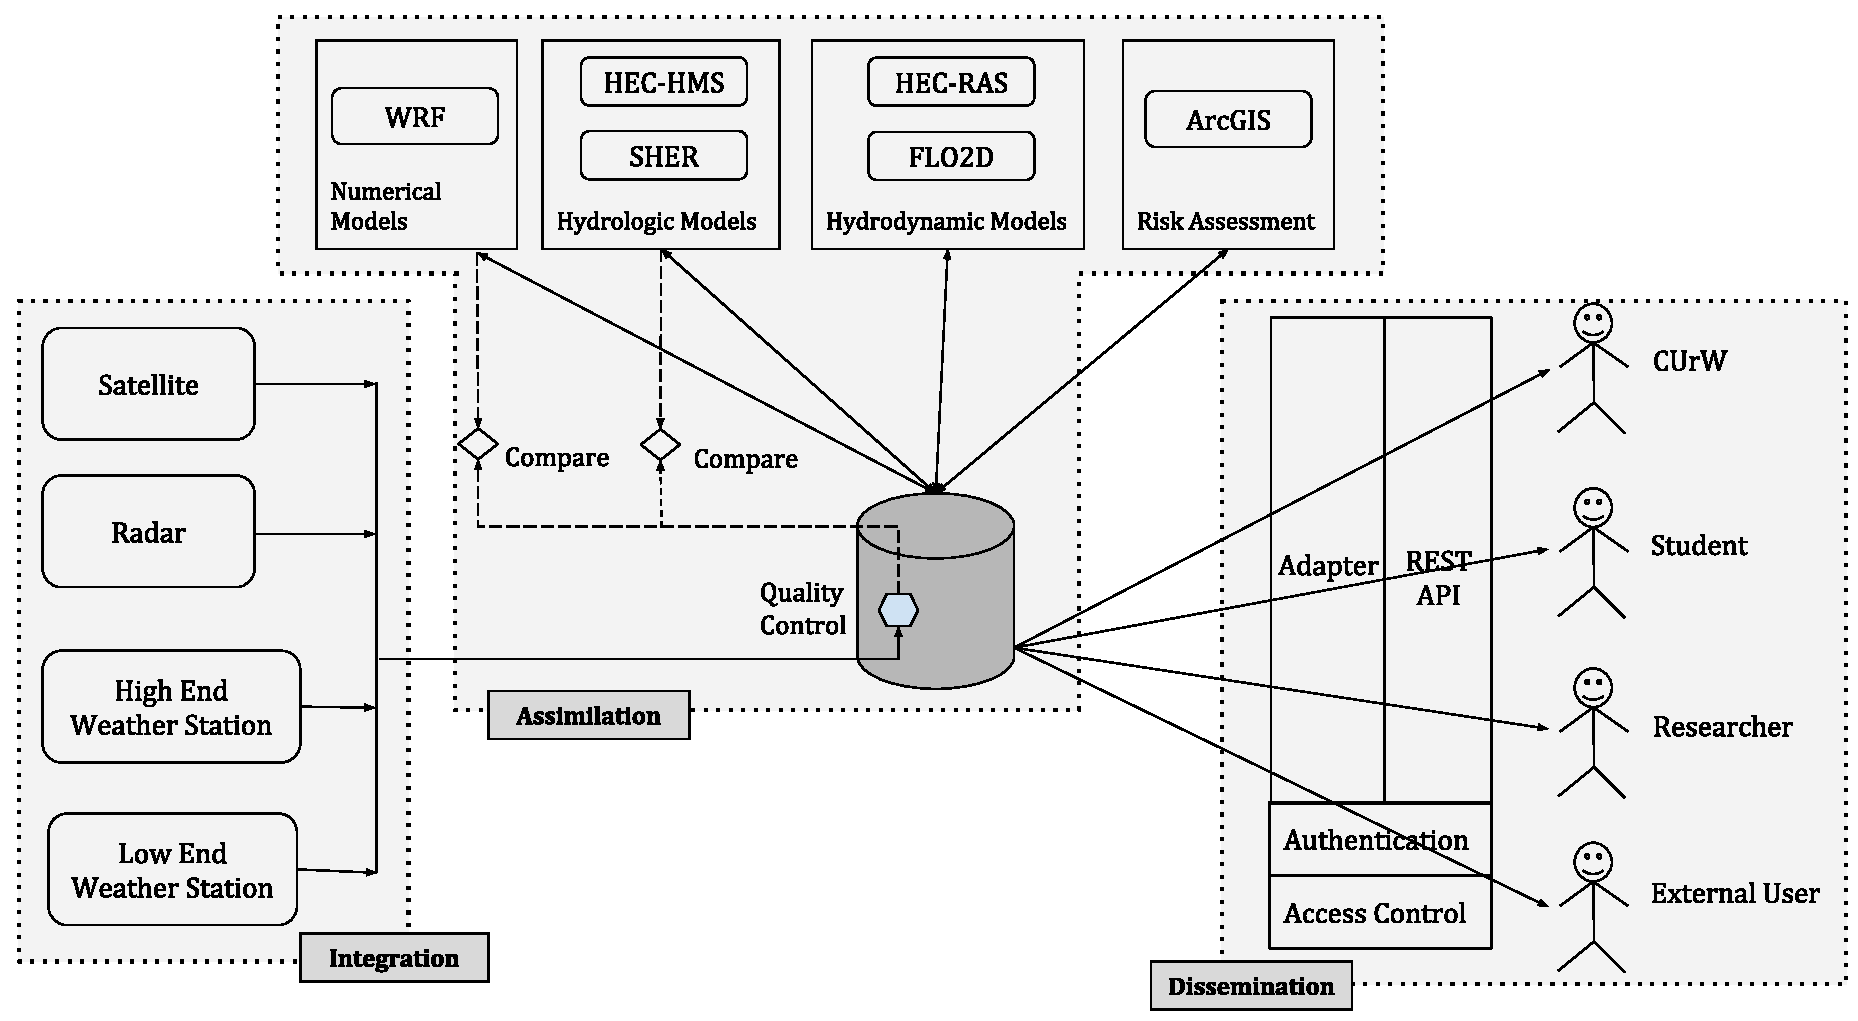
\includegraphics[width=0.5\textwidth]{images/weather_data_system_components_p1.pdf}}
\caption{Components of a weather data integration and assimilation system.}
\label{pfi:wdia_components}
\end{figure}

%\acrshort{wdias} supports all three modules shown in \cref{pfi:wdia_components}. While designing \acrshort{wdias}, we iterate through a few architectural designs to achieve high scalability and availability. Initially, we followed the \acrshort{soa} while using an \acrfull{esb} to integrate different modules. However, it turned out that we understood that \acrshort{esb} is not suitable for data streaming or bulk data processing and suffers from a single point of failure since it uses a common bus.
%In second design phase, we used the Actor model with AKKA framework with following the microservice architecture such that each microservice is implemented using actors. Microservice architecture is resilient and flexible as one service is independent of another service enables to highly scalable individual services. One of the attractive features of microservice architecture is the independent nature of the microservices which allows to choose different technologies and maintain separately. But using AKKA framework for implement microservice architecture has some disadvantages such as unable to choose independent technologies and the actors messaging between different services cause to result in a too-tight code coupling between the services.

%To overcome the issues using AKKA, we moved to the concept of container orchestration based microservice architecture. The \acrshort{wdias} used \acrfull{k8s} as the container orchestration system which is an open-source tool for automating deployment, scaling, and management of containerized applications. Using \acrshort{k8s}, users can add required resources as Nodes to the cluster, and K8s manage and deploy applications as pods into cluster nodes.
%In next \cref{pse:wdias_architecture}, we discussed about the \acrshort{wdias} used microservice concepts such as implement microservice as dumb pipes rather implementing smart endpoints, uses database per service with access via API only, distributed Transactions over microservices using event processing, and considering distributed systems scalability in directions of X-axis scaling, Y-axis scaling and Z-axis scaling.

%%%%%%%%%%%%%%%%%%%%%%%%%%%%%%%%%%%%%%%%%%%%%%%%%%%%%%%%%%%%%%%%%%%%%%%%%%%%%%%%
\section{Proposed Architecture}
\label{pse:wdias_architecture}

%%%%%%%%%%%%%%%%%%%%%%%%%%%%%%%%%%%%%%%%%%%%%%%%
\subsection{WDIAS Microservice Architecture}
\label{psubse:wdias_microservices}

\cref{pfi:wdia_components} shows the essential functions of a weather data integration and assimilation system such as integration, assimilation, and dissemination. A typical system should be capable of integrating multimodal and multidimensional spatial and temporal weather data from diverse sources such as satellites, radars, and high-end and low-end weather stations. In assimilation, the system not only stores the data but also provides them to various weather models in their desired data formats. In the dissemination step, both the captured weather data and processed data from weather models are shared with users and external systems based on their data subscriptions, timeseries metadata and geo-tag based queries, and access rights. \acrshort{wdias} supports all three of these modules.
\dbc{Is it "Microservice Architecture" or "Microservices Architecture"? It seems one with s is more common. Check this. Then makesure entire paper use one of this (including title).}
\gkc{I tried to follow these resources: https:\/\/martinfowler.com\/articles\/microservices.html. The term ''Microservice Architecture'' has sprung up over the last few years...}
\gkc{Here also refer as ''Microservice architecture'' : https:\/\/en.wikipedia.org\/wiki\/Microservices\#Introduction. If you think other is the correct one, we can change. Please let me know.}

%While designing \acrshort{wdias}, we iterated through a few architectural designs to achieve high scalability and availability. Initially, we followed the \acrshort{soa} while using an \acrfull{esb} to integrate different modules. However, it turned out that \acrshort{esb} is not suitable for data streaming and bulk data processing, as well as suffered from a single point of failure as it uses a common bus. We also attempted the Actor model with AKKA framework where each microservice was implemented using an actor. Microservice architectures were chosen as they are resilient, flexible, and scalable, as services were independent of each otehr. However, actors messaging between different services resulted in tight code coupling between the services and the platform was over dependent on the AKKA framework.
%To overcome these issues, we moved to container orchestration based microservices architecture. 
%The \acrshort{wdias} used \acrfull{k8s} as the container orchestration system which is an open-source tool for automating deployment, scaling, and management of containerized applications. Using \acrshort{k8s}, users can add required resources as Nodes to the cluster, and K8s manage and deploy applications as pods into cluster nodes.
%In next \cref{pse:wdias_architecture}, we discussed about the \acrshort{wdias} used microservice concepts such as implement microservice as dumb pipes rather implementing smart endpoints, uses database per service with access via API only, distributed Transactions over microservices using event processing, and considering distributed systems scalability in directions of X-axis scaling, Y-axis scaling and Z-axis scaling.

We used microservices architecture for \acrshort{wdias}, as it enables resilient and flexible services that can be independently scaled while achieving high-availability \cite{LewisMicroservices}. Such a design allows each module to be offered as a separate microservice where each module works on a separate piece of bulk or stream data. Microservices further enables modules to be written in any language and dynamically added to the system to extend its functionality. We implemented services as containerized applications, which further simplifies the deployment and maintenance of services on a cloud platform resulting in simplified administration and cost savings. \gk{Application containerization is an alternative to virtualization that encapsulate or group the software code and all its dependencies so that it can work uniformly and consistently in any infrastructure \cite{IBMContainerizationExplained}.The concept of containerization uses as an industry standard for package software into standardized units for development, shipment, and deployment.}
\dbc{Good to include a citation for microservices and containerization benefits.}
\gkc{Updated}

\begin{figure}[b!]
\centerline{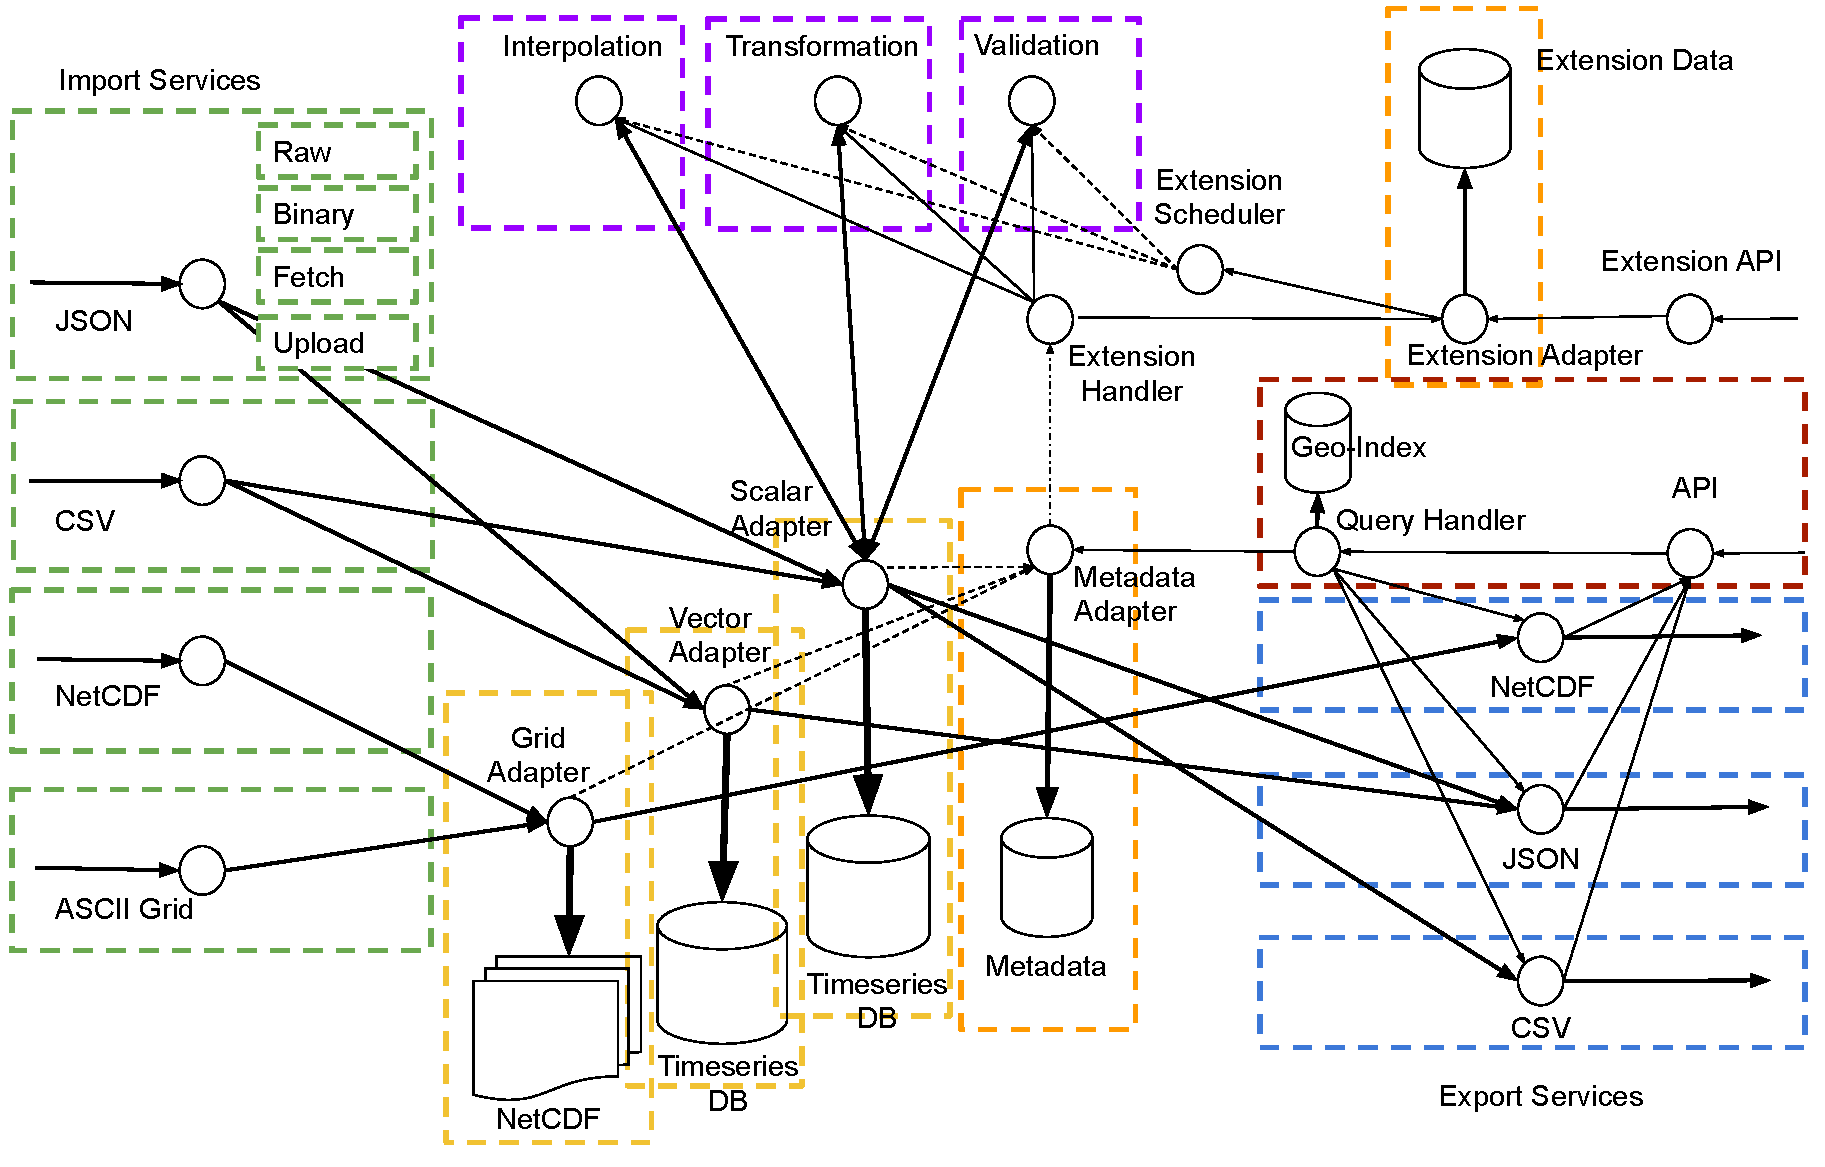
\includegraphics[width=0.5\textwidth]{images/separation_microservices-p1.pdf}}
\caption{Separation of \acrshort{wdias} microservices.}
\label{pfi:microservice_separation}
\end{figure}

\cref{pfi:microservice_separation} shows the separation of \acrshort{wdias}'s modules into the microservices where each circle represents a microservice. All microservices communicate using a RESTful API. Import modules are shown on left of figure while export modules are shown on right. Each import microservice coverts a specif type of data and forwards them to the relevant data adapter module which is optimized to store a specific type of data. Each adapter has an its own database instance enabling horizontal scalability. For example, timeseries metadata is stored in a relational database for faster querying. It can also be cased in an in-memory database to provide low-latency access. Similarly, export module microservices provide data to weather models and users while converting them to the desired format.
\dbc{We never mention about Raw, Binary, Fetch, and Upload. Also support for JSON, CSV, etc. Also, data transform operations are not metioned here (while they are given in II.3 we also need a sentence of 2 here. Extension Data, scheduler, etc. are not discussed either. 
We need to give a clear explanation of Fig. 2. So add a couple of sentences for these. Highlight them so that I can focus only on those sentences.}
\dbc{We should also touch about container solution and benefits such as scaling, and management of containerized applications. As we removed the entire para on Kubernetes (K8s) nothing is here now.}

% \begin{figure}[t!]
% \centerline{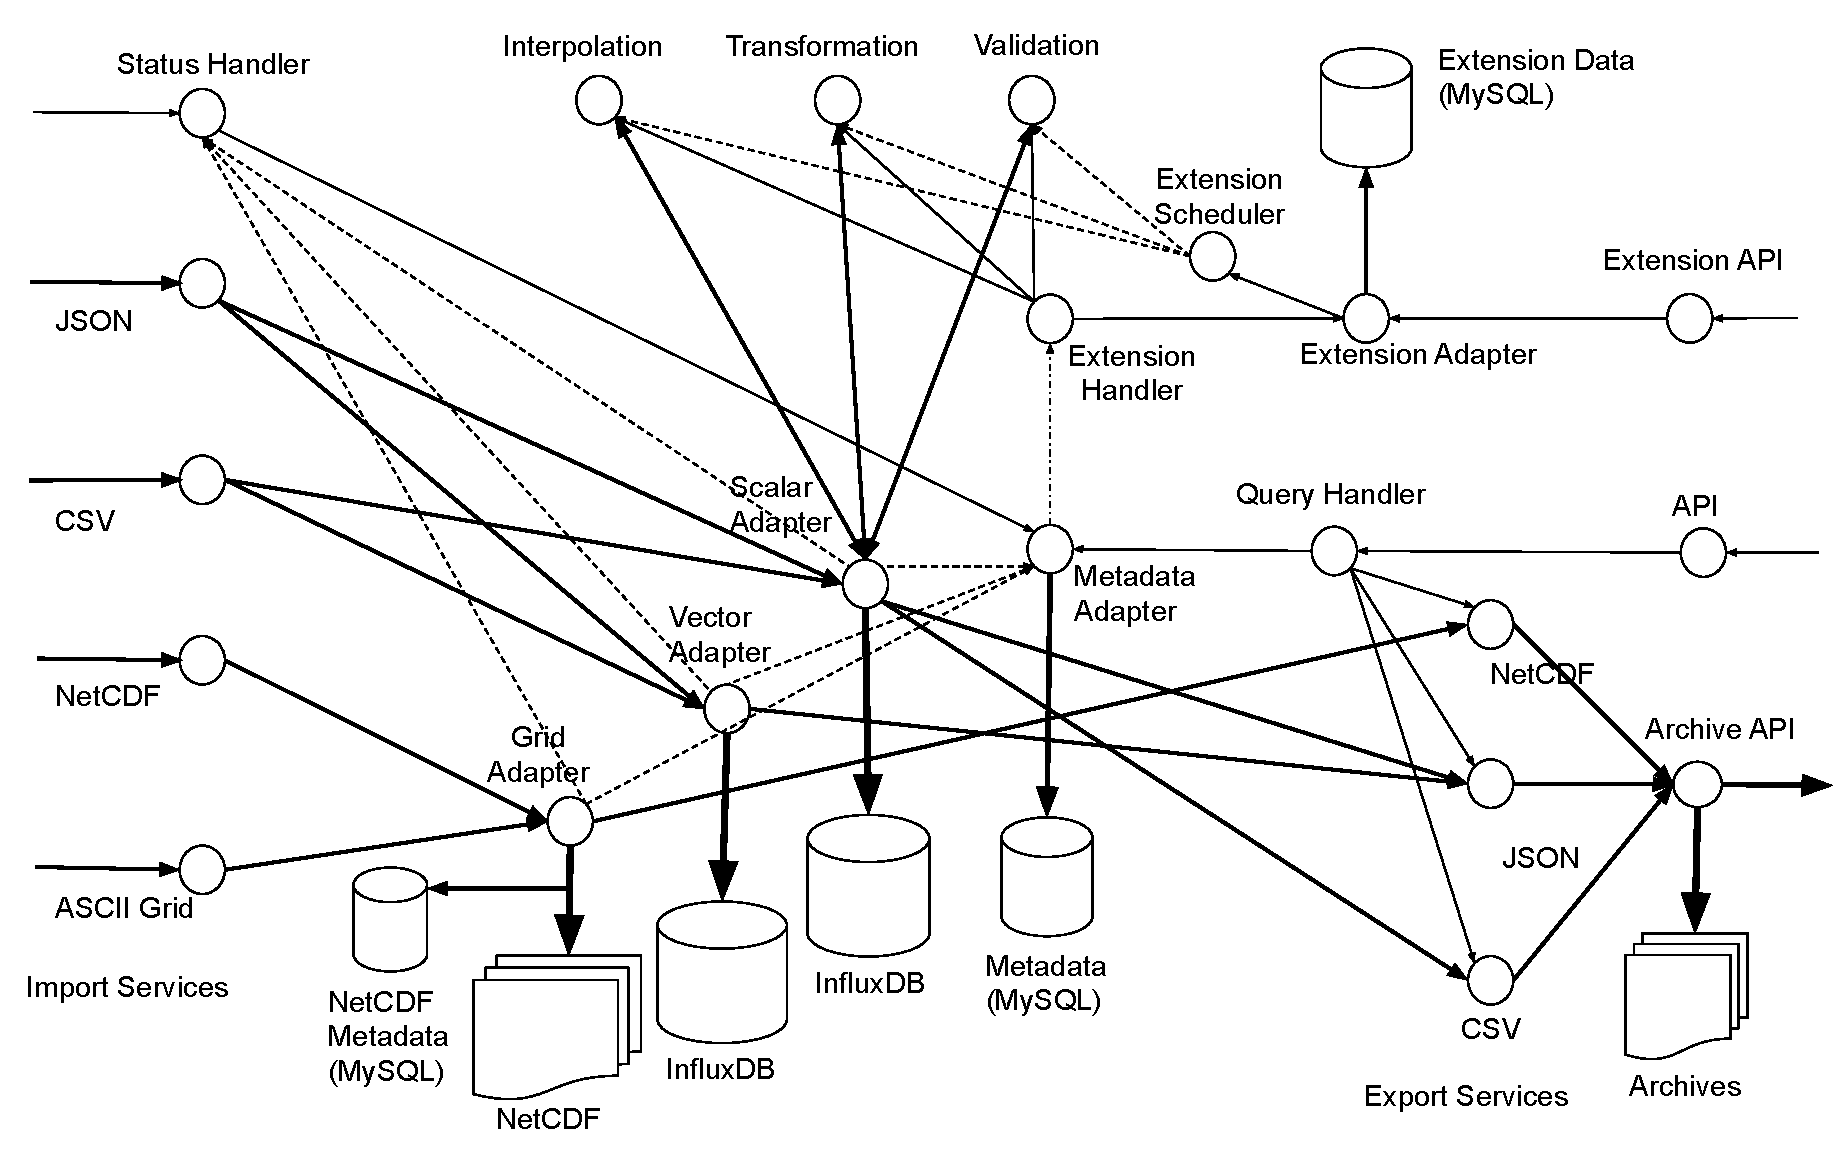
\includegraphics[width=0.5\textwidth]{images/microservice_architecture-handle_on_async-p1.pdf}}
% \caption{Asynchronously handling requests with microservices.}
% \label{pfi:microservice_architecture_async}
% \end{figure}

Each piece of data is tagged with a unique identifier (ID), which is used by all microservices to handle the data. A timeseries is considered as a single piece of data. Ingestion of a large piece of data, such as radar data in \acrfull{netCDF} format, is handled asynchronously. When a request with a large piece of data is received, rather than blocking the request, a unique ID is returned to the caller. This ID can be used later to verify successful processing of data or to download them.
% \db{As shown in \cref{pfi:microservice_architecture_async}, we use a Status Handler to manage the status of asynchronous requests. For example, when an ingestion module receives a large piece of data it is stored on the module. Then the module publishes an event to another service to process it. Once the successful processing of the data is verified, Status Handler updates the system status.}
\dbc{I updated the highlighted write up. But it doesn't make much sense. Also, it's not clear how to interpret the Fig. 3 (while it has some scattered lines, it not obvious what they do). If this is not essential let's remove highlighted text including figure. But you need to fix this on thesis for sure.}
\gkc{Lets remove this. It need more clarification. Since we have page limit, better to ignore this.}

%%%%%%%%%%%%%%%%%%%%%%%%%%%%%%%%%%%%%%%%%%%%%%%%
\subsection{Database Structure}
\label{psubse:wdias_database}

Timeseires are pervasive in weather domain from observations to forecasting. Thus, \acrshort{wdias} is designed to be data-centric with a special focus on timeseries data. Data points in a timeseries can consists of scalar (0D), vector (1D), grid (2D), and polygon (2D) data. We used the following list of metadata to uniquely identify a timeseirs:

\begin{itemize}
    \item \texttt{Module ID} -- is the source of data, e.g., weather station ID.
    \item \texttt{Location} -- that the data corresponds to, e.g., point locations and regular or irregular grid locations.
    \item \texttt{Value Type} -- indicates whether data consists of scalar, vector, grid, or polygon values.
    \item \texttt{Parameters} -- indicate the ambient measurements, e.g., temperature and pressure.
    \item \texttt{Timeseries Type} -- indicates whether the data is historical or forecast of a model.
    \item \texttt{Time Step} -- indicates the whether the sampling interval is uniform or not.
\end{itemize}

While a scalar data point consists of a single value, a vector data point consists of two values (e.g., magnitude and the direction of a vector). Whereas a grid data point consists of multiple values. Therefore, to manipulate data efficiently, as seen on \cref{pfi:database_structure} we used a combination of relational, NoSQL, timeseries, and in-memory databases, as well as flat files. He handle scalar and vector values using two different microservices, namely \textit{adapter-scalar} and \textit{adapter-vector} (see \cref{pfi:microservice_separation}), to isolate performance and faults. We used \acrshort{netCDF} files to store grid data as it is the de-factor standard for creating, accessing, and sharing of array-oriented scientific data. To resolve a query targeting timeseries data, we need to first identify the source and type of data, as well as where they are stored and what time or geographic range to retrieve. Hence, we used a relational database to manipulate timeseires metadata with low latency. We further used an in-memory database to enable low-latency query resolution by caching data stored in \textit{adapter-metadata} and \textit{adapter-extension} microservices. Further, spacial indexing (aka., geo-indexing) is needed to support queries based on the geo-location of data which are one of the hardest queries to resolve. Therefore, we used a document-oriented database for geo-indexing and searching.
\dbc{We should also mention briefly why we selected InfluxDB, MySQL, in-memory (what's the product?), and NoSQL (what's the product)}

\begin{figure}[t!]
\centerline{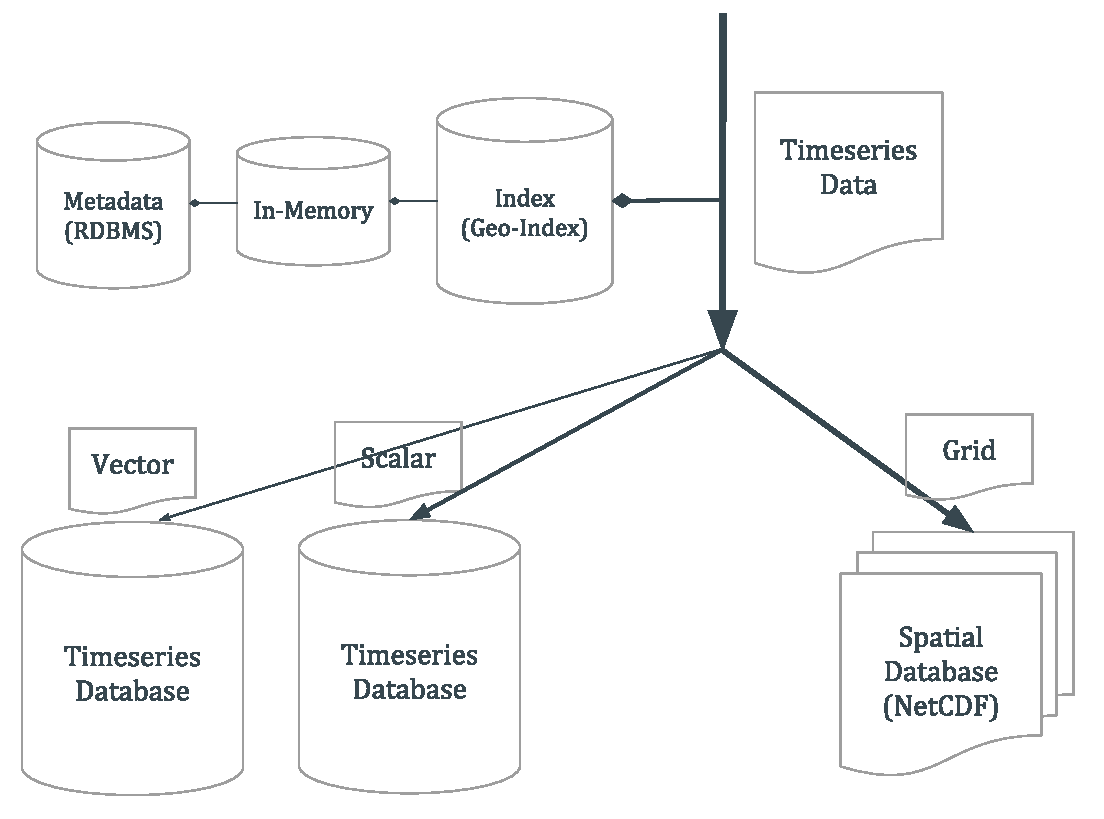
\includegraphics[width=0.4\textwidth]{images/wdias_database_structure_p1.pdf}}
\caption{\acrshort{wdias} database structure.}
\label{pfi:database_structure}
\end{figure}
\dbc{Fig. 4 looked washed out. Make lines black.}



%%%%%%%%%%%%%%%%%%%%%%%%%%%%%%%%%%%%%%%%%%%%%%%%
\subsection{Data Preprocessing}
\label{psubse:data_preprocessing}

\acrshort{wdias} provides the data preprocessing capabilities via extension modules. As seen in \cref{pfi:summary_weather_data_preprocessing} each extension could be considered as a mathematical function that takes \texttt{p} timeseries variables as input and output \texttt{n} timeseries variables. As seen on bottom half of figure, these functions are typically used for data quality checks, interpolation (both serial and spatial), and transformation. To further extend the function at run time without creating a new module, the \textit{bind constant} can be set at the time of triggering an extension. For example, such features are needed as we may need to generate two different timeseries by sub-sampling 1-minute data to 5 minutes and one hour. While this increases the data stored by \acrshort{wdias}, it reduces the computational time as NWMs can readily use the data without transforming them at the run time. \cref{pli:extension_triggers} shows the format of a request made to update an extension at the time of triggering it. Each extension trigger needs to have a unique ID (line 2). Then the user can define the extension type and the microservice responsible of processing it (lines 3 and 4). Using lines 5-12 the user can map timeseries into input variable \emph{X} and output variablr \emph{Y} as seen in \cref{pfi:summary_weather_data_preprocessing}. Finally, user can also define when to trigger the extension and any options such as bind constant. Using different update requests \acrshort{wdias} can create multiple triggers for an extension. The \emph{Extension Handler} is responsible for triggering the correct extension when there is a change on the subscribed extension trigger's \emph{OnChange} timeseries. 
\dbc{We never talked about a \emph{OnChange} timeseries.}

\begin{figure}[t!]
\centerline{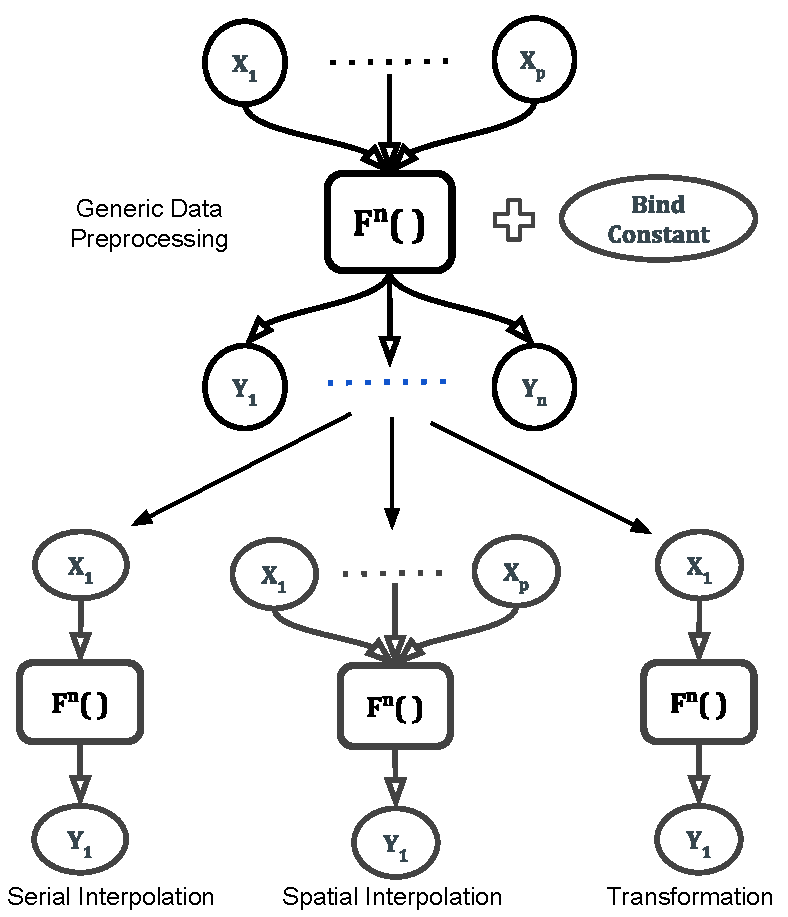
\includegraphics[width=0.4\textwidth]{images/summary_weather_data_preprocessing_p1.pdf}}
\caption{Functional approach to weather data preprocessing.}
\label{pfi:summary_weather_data_preprocessing}
\end{figure}


\begin{lstlisting}[language=Python, caption=Format of a request made to update an extension., label=pli:extension_triggers]
{
    "extensionId": "", //Trigger unique ID
    "extension": "Interpolation | Transformation | Validation",
    "function": "", //Mapping microservice
    "variables": [ //Timeseries mapping to variables
        {
            "variableId": "",
            "metadata/metadtaIds": {...}
        }
    ],
    "inputVariables": [], //Input timeseries
    "outputVariables": [], //Output timeseries
    "trigger": [ // When to trigger the function
        {
            "trigger_type": "OnChange | OnTime",
            "trigger_on": []
        }
    ],
    "options": { //Run time bind constant data
    }
}
\end{lstlisting}


%\emph{Extension Handler} is responsible for triggering the correct Extension with metadata at a given time which is provided at the creation on extension trigger with the value of \emph{OnTime} cronjob string value. To improve the performance of triggering cronjobs at given time schedules, the WDIAS added few optimization mechanisms.

%%%%%%%%%%%%%%%%%%%%%%%%%%%%%%%%%%%%%%%%%%%%%%%%
\subsection{Query Resolution}
\label{psubse:query_timeseries}

% \acrshort{wdias} supports both timeseries and geo-location based queries. For example, it can query for a timeseries in a given area. This operation uses \texttt{geoWithin} search operator for the simplicity. Other than it can also support query timeseries in an area by parameter, query available timeseries by locations and query locations within an area etc. In \cref{pli:geo_search}, the \acrshort{wdias} return the timeseries available within the area of a polygon provided as \emph{geoJson} \cite{InternetEngineeringTaskForceGeoJSON}.
Other than the metadata manipulation API mentioned in \cref{psubse:wdias_microservices}, the \acrshort{wdias} also supports timeseries search queries and Geo queries. As an example it can \emph{query timeseries available in a given area}. This operation uses \texttt{geoWithin} search operator for the simplicity. Other than it can also support query timeseries in an area by parameter, query available timeseries by locations and query locations within an area of a polygon provided as \emph{geoJson} \cite{InternetEngineeringTaskForceGeoJSON}.
\dbc{This section need a bit of expansion. Also, discuss who issue these queries and how the results are sent out. As we don't have a section on Export serveries they can be covered here. Perhaps even changing the name of the sub-section is an option.}
\dbc{What's \texttt{geoWithin}?}
\dbc{Drop Listing 2 as it's not essential.}
 
% \begin{lstlisting}[caption=Geo search timeseries, label=pli:geo_search]
%     POST <HOST_NAME>/query/timeseries
%     JSON Body:
%     {
%         "geoJson": {
%             "type": "Polygon",
%             "coordinates": [
%                 [
%                     [<longitude>, <latitude>],
%                     ...
%                 ]
%             ]
%         }
%     }
% \end{lstlisting}

%%%%%%%%%%%%%%%%%%%%%%%%%%%%%%%%%%%%%%%%%%%%%%%%%%%%%%%%%%%%%%%%%%%%%%%%%%%%%%%%
\section{Performance Analysis}
\label{pse:performance_analysis}

%%%%%%%%%%%%%%%%%%%%%%%%%%%%%%%%%%%%%%%%%%%%%%%%
\subsection{Experimental Setup}
\label{psubse:experimental_setup}

%The test plan is to perform load testing on whole system, and analyze the scalability of the system while measuring the operations perform on each module. Two variables can vary while doing performance testing.
%\begin{enumerate}
%    \item \acrfull{rps}
%    \item Request size
%\end{enumerate}

As a weather data integration and assimilation system is expected to handle variety of data sources and types, we created a synthetic workload consisting of 70\% scalar, 20\% vector, and 10\% grid values. 
We created 1,000 timeseries using 30-day traces from five weather stations of \acrlong{curw}. Locations of timeseries were set based on the Google's Countries dataset \cite{GoogleGoogleCounties}. For grid data we considered a grid size of 100. 
\dbc{Clearly mention what weather attributes we used and how we build a 1000 timeseries using only 5 weather stations. This should also cover how vector and grid values were generated.}
\dbc{When referring to tables T should be capital}

Load testing was performed using Apache JMeter with distributed testing feature, which use multiple workload generators to create a high throughput workload. We vary the request size by varying the resolution of data expected from the system, e.g., we requested aggregated data for an hour, 30 minutes, and 15 minutes. For a given request size, we issued requests at different rates such as 10, 50, 100, 200, and 600 requests per second. For a given combination of request size and rate, we tested the system for 30 minutes. We then moved to a more demanding combination of request size and rate to measure effectiveness of auto scaling of the container orchestration system. After reaching the highest request size and rate combination, we also measured how the system will gradually release the resources when there is not load on the system. 
\dbc{What's a request here, ingest or export? While I see Insert, Retrieve, Query in tables, we are not clearly explaining them here.}
\dbc{Given that we had a mix of 70 : 20 : 10 requests what's mean by request size is not quite clear (I updated above sentence, but still feel like we are not clearly explaining it)?}
\dbc{After modifying I ended up this part of sentence ``and perform 5minutes test run with timeseries queries.'' which I was not clear how to edit} 
\dbc{Be clear that aggregation of 1H, 30min, and 15min was done only for Retrieve requests.}

\acrshort{wdias} was deployed using \acrfull{eks} container orchestration platform. \cref{ptab:aws_eks_nodes} shows the list of nodes used in the experimental setup. \db{\emph{Core} node executed metadata, extensions, query, status and extension microservices. Whereas the \emph{grid} node executed the grid adapter, as well as grid data import and export services. Scalar and vector adapters, as well as scalar and vector import and export services were deployed on the \emph{scalar} node. JMeter and metric server executed on the \emph{test} node.} Given a set of computing resources, to get the better performance, we scheduled each microservice on a predefined set of nodes.
\dbc{Some of the terms in highlighted part was never mentioned in text. Hence, it's important that these are introduced in Sec. II.A}

\db{WDIAS, uses the Concurrency Thread Group with Throughput Shaping Timer because it supports the open workload approach.}
\dbc{Highlighted sentence is not clear to me.}

\begin{itemize}
    \item \emph{closed system model} \cite{Haggett1998AnWales} -- a new request is only triggered by the completion of a previous request, following by a think time.
    \item \emph{open system model} -- new requests arrival independently of completions.
\end{itemize}
\dbc{What are these?}

\dbc{From Table II to V it seems we separated out timeseries and grid requests. Also, there are Insert, Retrieve, and query requests. These need to be clearly mentioned in this sub-section to avoid any confusion.}

\begin{table}[tb!]
\caption{\acrshort{eks} nodes}
\begin{center}
\begin{adjustbox}{width=0.45\textwidth}
\begin{tabular}{|l|r|r|r|r|l|}
\hline
\textbf{Node} & \textbf{vCPUs} & \textbf{RAM (GB)} & \textbf{Storage (GB)} & \textbf{Quantity} & \textbf{EC2 Name} \\ \hline
core & 16 & 32 & 15 & 1 & c5.4xlarge \\ \hline
grid & 8 & 16 & 25 & 1 & c5.2xlarge \\ \hline
scalar & 8 & 16 & 20 & 1 & c5.2xlarge \\ \hline
test & 4 & 10.5 & 5 & 1 & c5n.xlarge \\ \hline
\end{tabular}
\end{adjustbox}
\label{ptab:aws_eks_nodes}
\end{center}
\end{table}



%%%%%%%%%%%%%%%%%%%%%%%%%%%%%%%%%%%%%%%%%%%%%%%%
\subsection{Performance Evaluation}
\label{psubse:performance_evaluation}

\cref{ptab:obs_all_60_min_summary_throughput} to \cref{ptab:obs_all_15_min_summary_throughput} show the throughput (measured as \acrlong{rps}), latency, and errors under three different data resolutions with a fixed service setup. Whereas \cref{ptab:obs_all_auto_15_min_summary_throughput} shows the performance with the container auto-scaling. It can be seen that each test resulted in approximately 310K requests within 30 minutes. Avg., 90\%, and STD indicates the average, standard deviation, and 90\% percentile for latency.  Other than some grid timeseries inserts, all other operations succeed with no errors.

\dbc{What's the request rate when collecting data for Tables II to V?}
\dbc{It seems you are using RPS to indicate throughput, which is the rate that we make requests not the rate that system responds. However, if latency is low and requests don't pile up we can say system can handle this request rate. We need to be a bit clear on this.}

From \cref{ptab:obs_all_60_min_summary_throughput} to \cref{ptab:obs_all_15_min_summary_throughput} it can be seen that the average and 90\% percentile latency to insert scalar and vector timeseries increased by 2 ms and 10 ms, respectively as we increase the request size. Still \acrshort{wdias} was able to accept 40.5 \acrshort{rps}. However, while retrieving the scalar and vector timeseries data, latency got doubled while handling the 15-min data compared to 30-min data. \db{This is due to heavy writes on the timeseries database.} However, there is no noticeable reduction in RPS. Therefore, even through the data volume increased by four times, \acrshort{wdias} performance degradation is sub-linear. 

\dbc{How come heavy writing happens when retrieving data? Shouldn't it happen during ingestion. Or is it because we are running data preprocessing at the time of request? This need to be clearly explained.}

\begin{table}[tb!]
\centering
\caption{Performance while processing 60-min data requests.}
\begin{adjustbox}{width=0.45\textwidth}
% \footnotesize
\begin{tabular}{|l|r|r|r|r|r|r|}
\hline
\textbf{Request Type} & \textbf{\# Samples} & \textbf{RPS} & \textbf{Avg.} & \textbf{90\%} & \textbf{STD} & \textbf{Error \%} \\ \hline
Insert Timeseries & 71826 & 40.5 & 28 & 31 & 58.74 & 0.00\% \\ \hline
Retrieve Timeseries & 71796 & 40.7 & 8 & 10 & 4.18 & 0.00\% \\ \hline
Insert Grid & 7982 & 4.5 & 23 & 26 & 4.23 & 0.06\% \\ \hline
Retrieve Grid & 7979 & 4.5 & 68 & 75 & 10.11 & 0.00\% \\ \hline
Query Location & 71804 & 40.5 & 3 & 3 & 1.52 & 0.00\% \\ \hline
\textbf{TOTAL} & 311182 & 175.4 & 127 & 503 & 207.80 & 0.00\% \\ \hline
%\multicolumn{4}{l}{$^{\mathrm{a}}$S.D.: Standard Deviation}{$^{\mathrm{b}}$90\%: 90\% percentile}
\end{tabular}
\end{adjustbox}
\label{ptab:obs_all_60_min_summary_throughput}
\end{table}

\dbc{We need to use a more meaningful term than ``60-min data'', ``30-min data', and ``15-min data'' because these reflect only the size of Retrieve requests. If this also indicates Insert timeseries' sampling interval, we need to clearly mention this in Sec. III.A}

\begin{table}[tb!]
\caption{Performance while processing 30-min data requests.}
\begin{center}
\begin{adjustbox}{width=0.45\textwidth}
% \footnotesize
\begin{tabular}{|l|r|r|r|r|r|r|}
\hline
\textbf{Request Type} & \textbf{\# Samples} & \textbf{RPS} & \textbf{Avg.} & \textbf{90\%} & \textbf{STD} & \textbf{Error \%} \\ \hline
Insert Timeseries & 71759 & 40.5 & 29 & 32 & 50.97 & 0.00\% \\ \hline
Retrieve Timeseries & 71730 & 40.6 & 9 & 10 & 6.04 & 0.00\% \\ \hline
Insert Grid & 7972 & 4.5 & 44 & 49 & 8.17 & 0.08\% \\ \hline
Retrieve Grid & 7971 & 4.5 & 81 & 93 & 15.15 & 0.00\% \\ \hline
Query Location & 71734 & 40.5 & 3 & 3 & 1.90 & 0.00\% \\ \hline
TOTAL & 310878 & 175.3 & 129 & 0 & 207.10 & 0.00\% \\ \hline
%\multicolumn{4}{l}{$^{\mathrm{a}}$S.D.: Standard Deviation}{$^{\mathrm{b}}$90\%: 90\% percentile}
\end{tabular}
\end{adjustbox}
\label{ptab:obs_all_30_min_summary_throughput}
\end{center}
\end{table}

Latency to insert grid timeseries data is relatively low compared to scalar or vector inserts as grid data are handled asynchronously. When the number of grid files doubled, latency also doubled as \db{....} \db{Yet, \acrshort{wdias} was able to handle the all the incoming requests.}
\dbc{We need to talk about why errors increased.}
\dbc{Explain why when the number of grid files double, latency also double. Is it because twice the bandwidth is needed?}
\db{Retrieving of Grid timeseries data happens on demand during the load test. But it is possible to upgrade the system to support asynchronously download alongside with direct download. Because of that, the latency of download the the Grid data is bit higher than the other test cases.}
\dbc{Highlighted text is not clear to me. Also, I'm confused about how asyn cases are handled for Insert and Retrieve. Did you measure latency to get only the unique ID or entire data?}

\begin{table}[tb!]
\caption{Performance while processing 15-min data requests.}
\begin{center}
\begin{adjustbox}{width=0.45\textwidth}
% \footnotesize
\begin{tabular}{|l|r|r|r|r|r|r|}
\hline
\textbf{Request Type} & \textbf{\# Samples} & \textbf{RPS} & \textbf{Avg.} & \textbf{90\%} & \textbf{STD} & \textbf{Error \%} \\ \hline
Insert Timeseries & 71775 & 40.5 & 30 & 41 & 51.71 & 0.00\%  \\ \hline
Retrieve Timeseries & 71736 & 40.6 & 23 & 32 & 50.18 & 0.00\%  \\ \hline
Insert Grid & 7975 & 4.5 & 91 & 112 & 19.58 & 1.42\% \\ \hline
Retrieve Grid & 7972 & 4.5 & 118 & 165 & 56.15 & 0.00\% \\ \hline
Query Location & 71749 & 40.5 & 3 & 4 & 2.32 & 0.00\% \\ \hline
\textbf{TOTAL} & 310934 & 175.4 & 134 & 503 & 206.40 & 0.04\% \\ \hline
%\multicolumn{4}{l}{$^{\mathrm{a}}$S.D.: Standard Deviation}{$^{\mathrm{b}}$90\%: 90\% percentile}
\end{tabular}
\end{adjustbox}
\label{ptab:obs_all_15_min_summary_throughput}
\end{center}
\end{table}

In all test cases, performance in resolving location-based queries remained the same. This was due to the geo-index build using the NoSQL database. 
\dbc{When we change from 1H to 15min, was there any impact on location queries? My understanding is there no such change unless queries were issued more frequently (this seems to be not the case from 3 tables) or queries asked for more data?}
% To get better performance test on the query module, we performed set of complex queries as shown in the \cref{ptab}

\begin{table}[tb!]
\caption{Performance while processing 60-min data requests when auto-scaling is enabled.}
\begin{center}
\begin{adjustbox}{width=0.45\textwidth}
\footnotesize
\begin{tabular}{|l|r|r|r|r|r|r|}
\hline
\textbf{Request Type} & \textbf{\# Samples} & \textbf{RPS} & \textbf{Avg.} & \textbf{90\%} & \textbf{STD} & \textbf{Error \%}\\ \hline
Insert Timeseries & 71727 & 40.5 & 34 & 27 & 118.78 & 0.00\% \\ \hline
Retrieve Timeseries & 71693 & 40.5 & 7 & 9 & 18.72 & 0.00\% \\ \hline
Insert Grid & 7968 & 4.5 & 87 & 98 & 14.07 & 0.18\% \\ \hline
Retrieve Grid & 7965 & 4.5 & 89 & 110 & 37.79 & 0.00\% \\ \hline
Query Location & 71704 & 40.5 & 1 & 2 & 2.05 & 0.00\% \\ \hline
\textbf{TOTAL} & 310734 & 175.3 & 130 & 501 & 212.35 & 0.00\% \\ \hline
%\multicolumn{4}{l}{$^{\mathrm{a}}$S.D.: Standard Deviation}{$^{\mathrm{b}}$90\%: 90\% percentile}
\end{tabular}
\end{adjustbox}
\label{ptab:obs_all_auto_15_min_summary_throughput}
\end{center}
\end{table}

\cref{ptab:obs_all_auto_15_min_summary_throughput} shows the performance when we enabled container auto-scaling. When we were inserting and retrieving data at 15-min resolution, microservices handling grid data had high resource utilization and 1.4\% of the grid insert requests failed. Once the auto-scaling was enabled, resource utilization of microservices were balanced. This reduced both the errors (0.18\%) and the overall latency for inserting and retrieving grid data.

\begin{figure}[b!]
\centerline{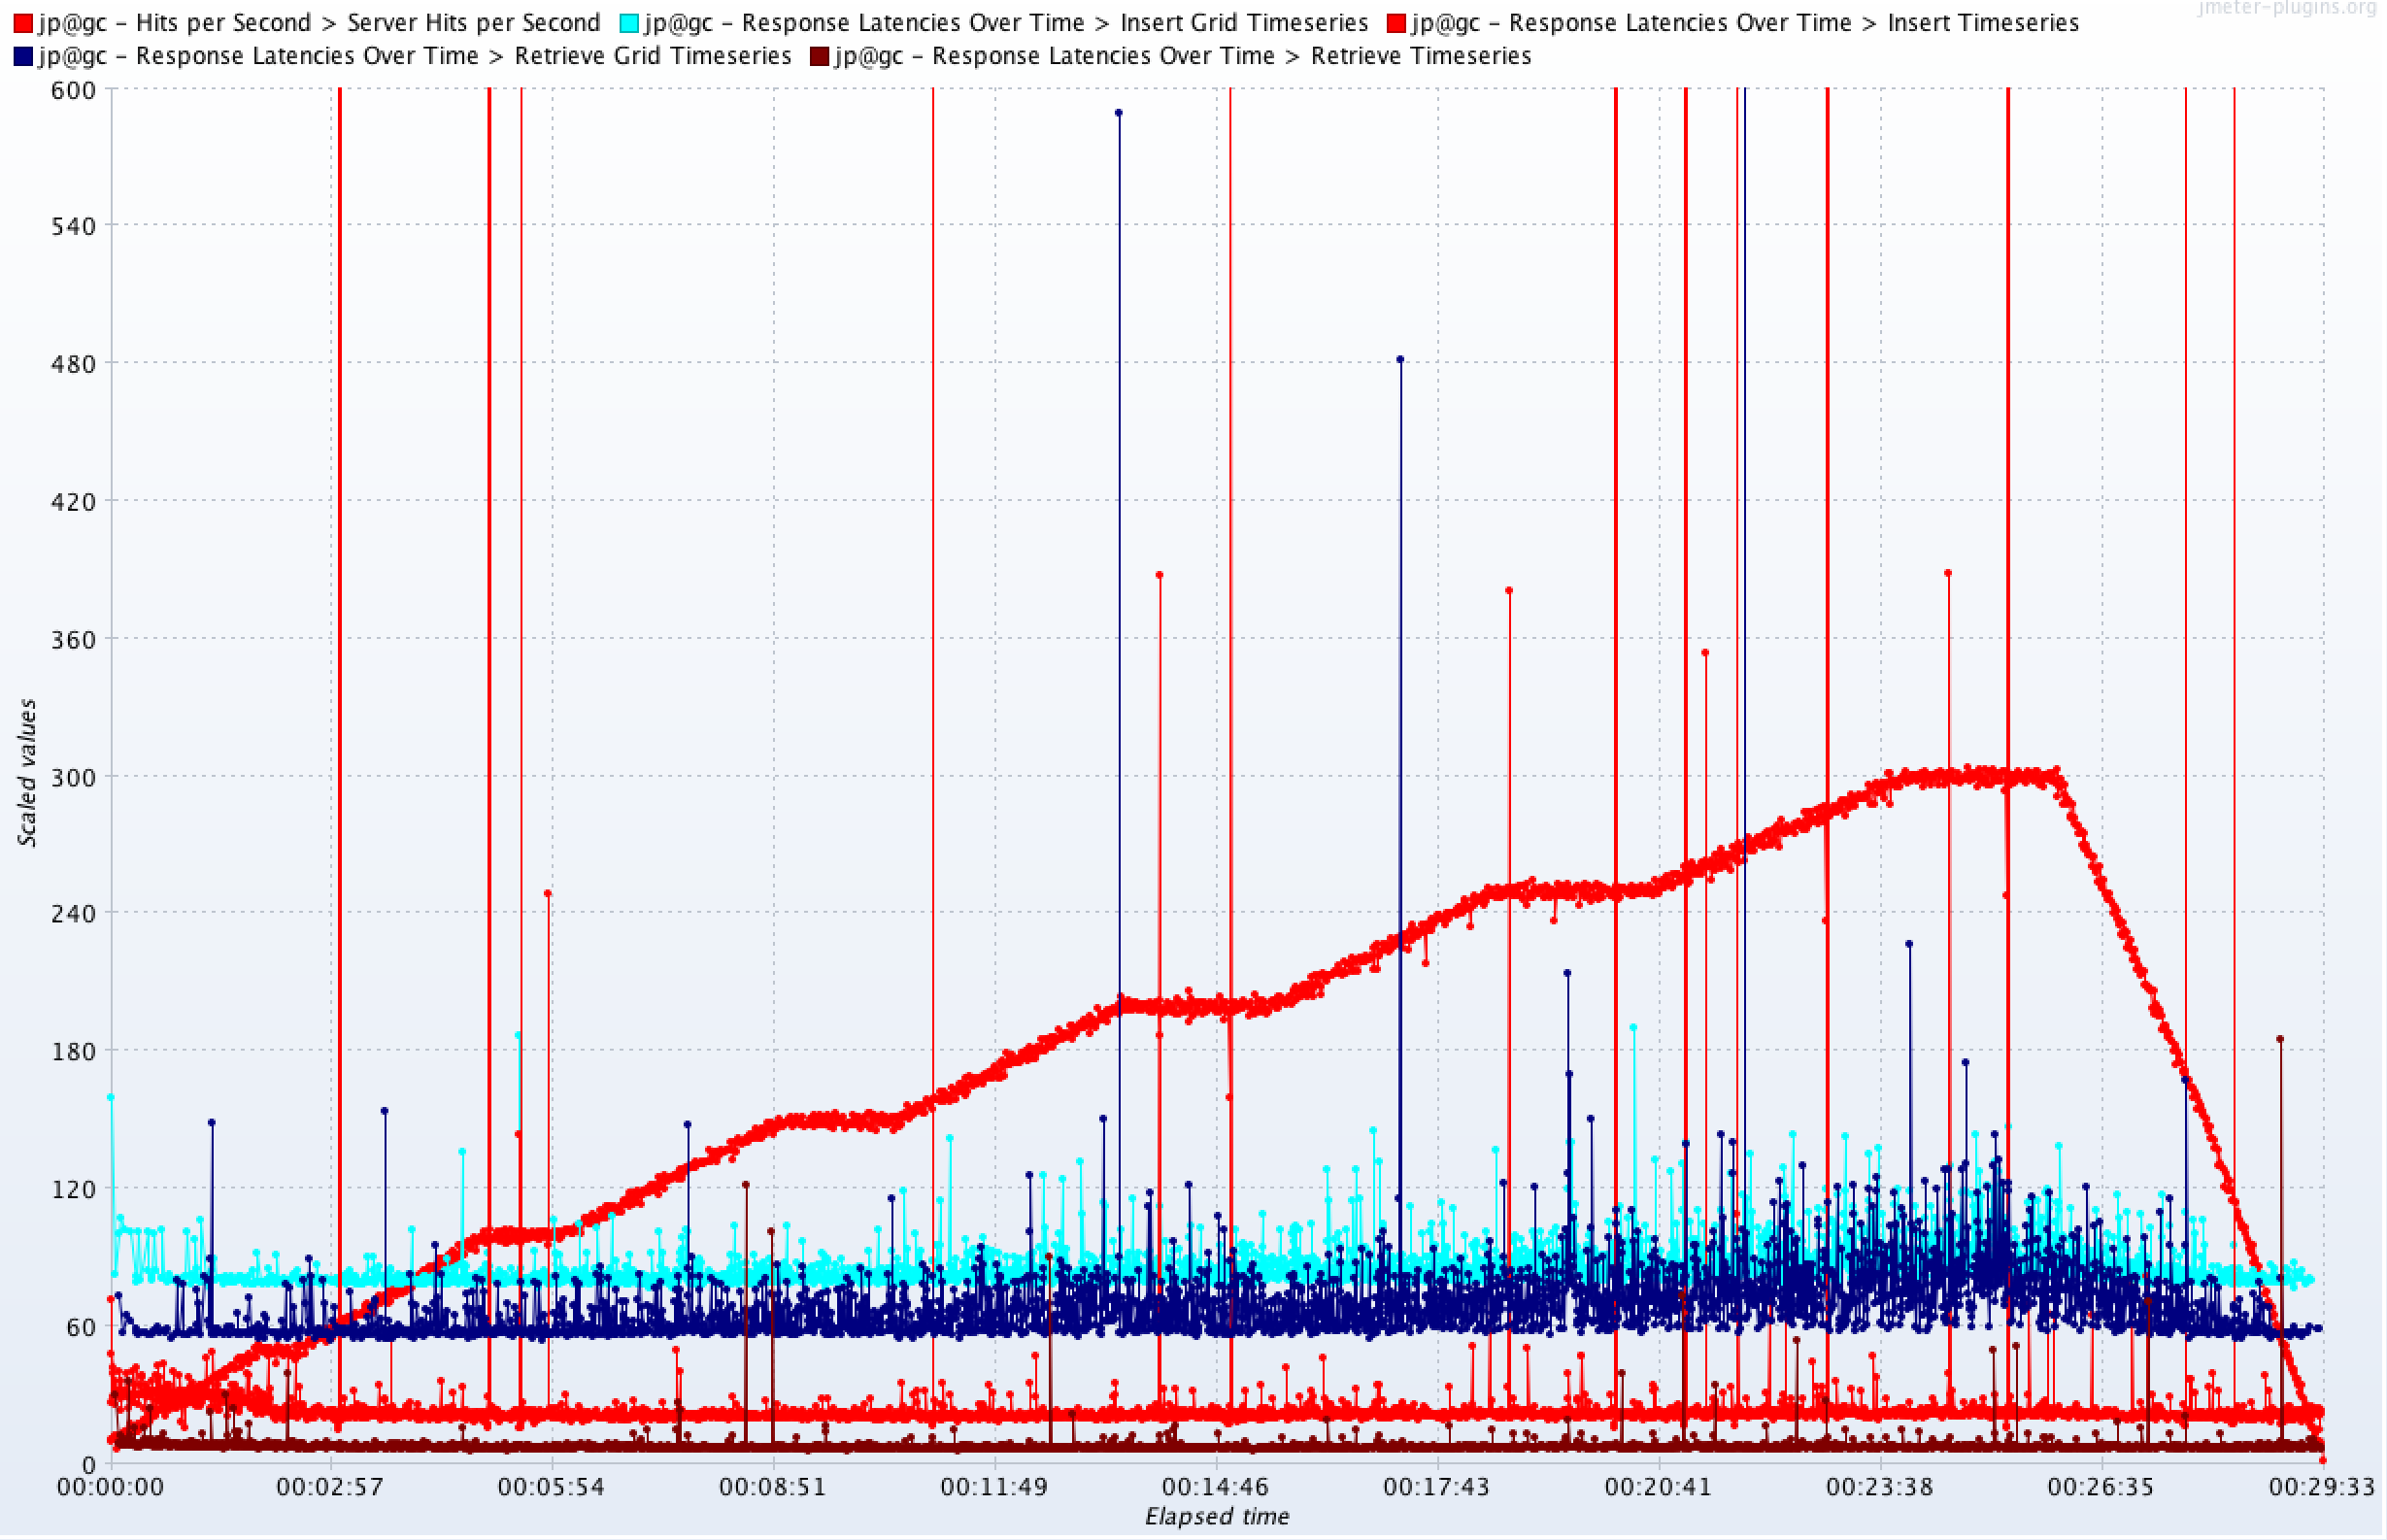
\includegraphics[width=0.5\textwidth]{results/obs/all_auto/obs_all_auto_15m_res_latencies_against_hits.png}}
\caption{Variation of request rate and latency with elapsed time with auto-scaling and 15-min data.}
\label{pfi:test_obs_auto_all_15_min_latency_vs_hits}
\end{figure}

\cref{pfi:test_obs_auto_all_15_min_latency_vs_hits} shows the latency of each request type under 15-min resolution and auto-scaling. Even through the request rate increased linearly (indicated by red line), no significant increase in latency was observed for request types other than grid data related requests (indicated by blue line). Even then, latency was within $2\times$ while the request rate was $5\times$.

%\begin{figure}[t!]
%\centerline{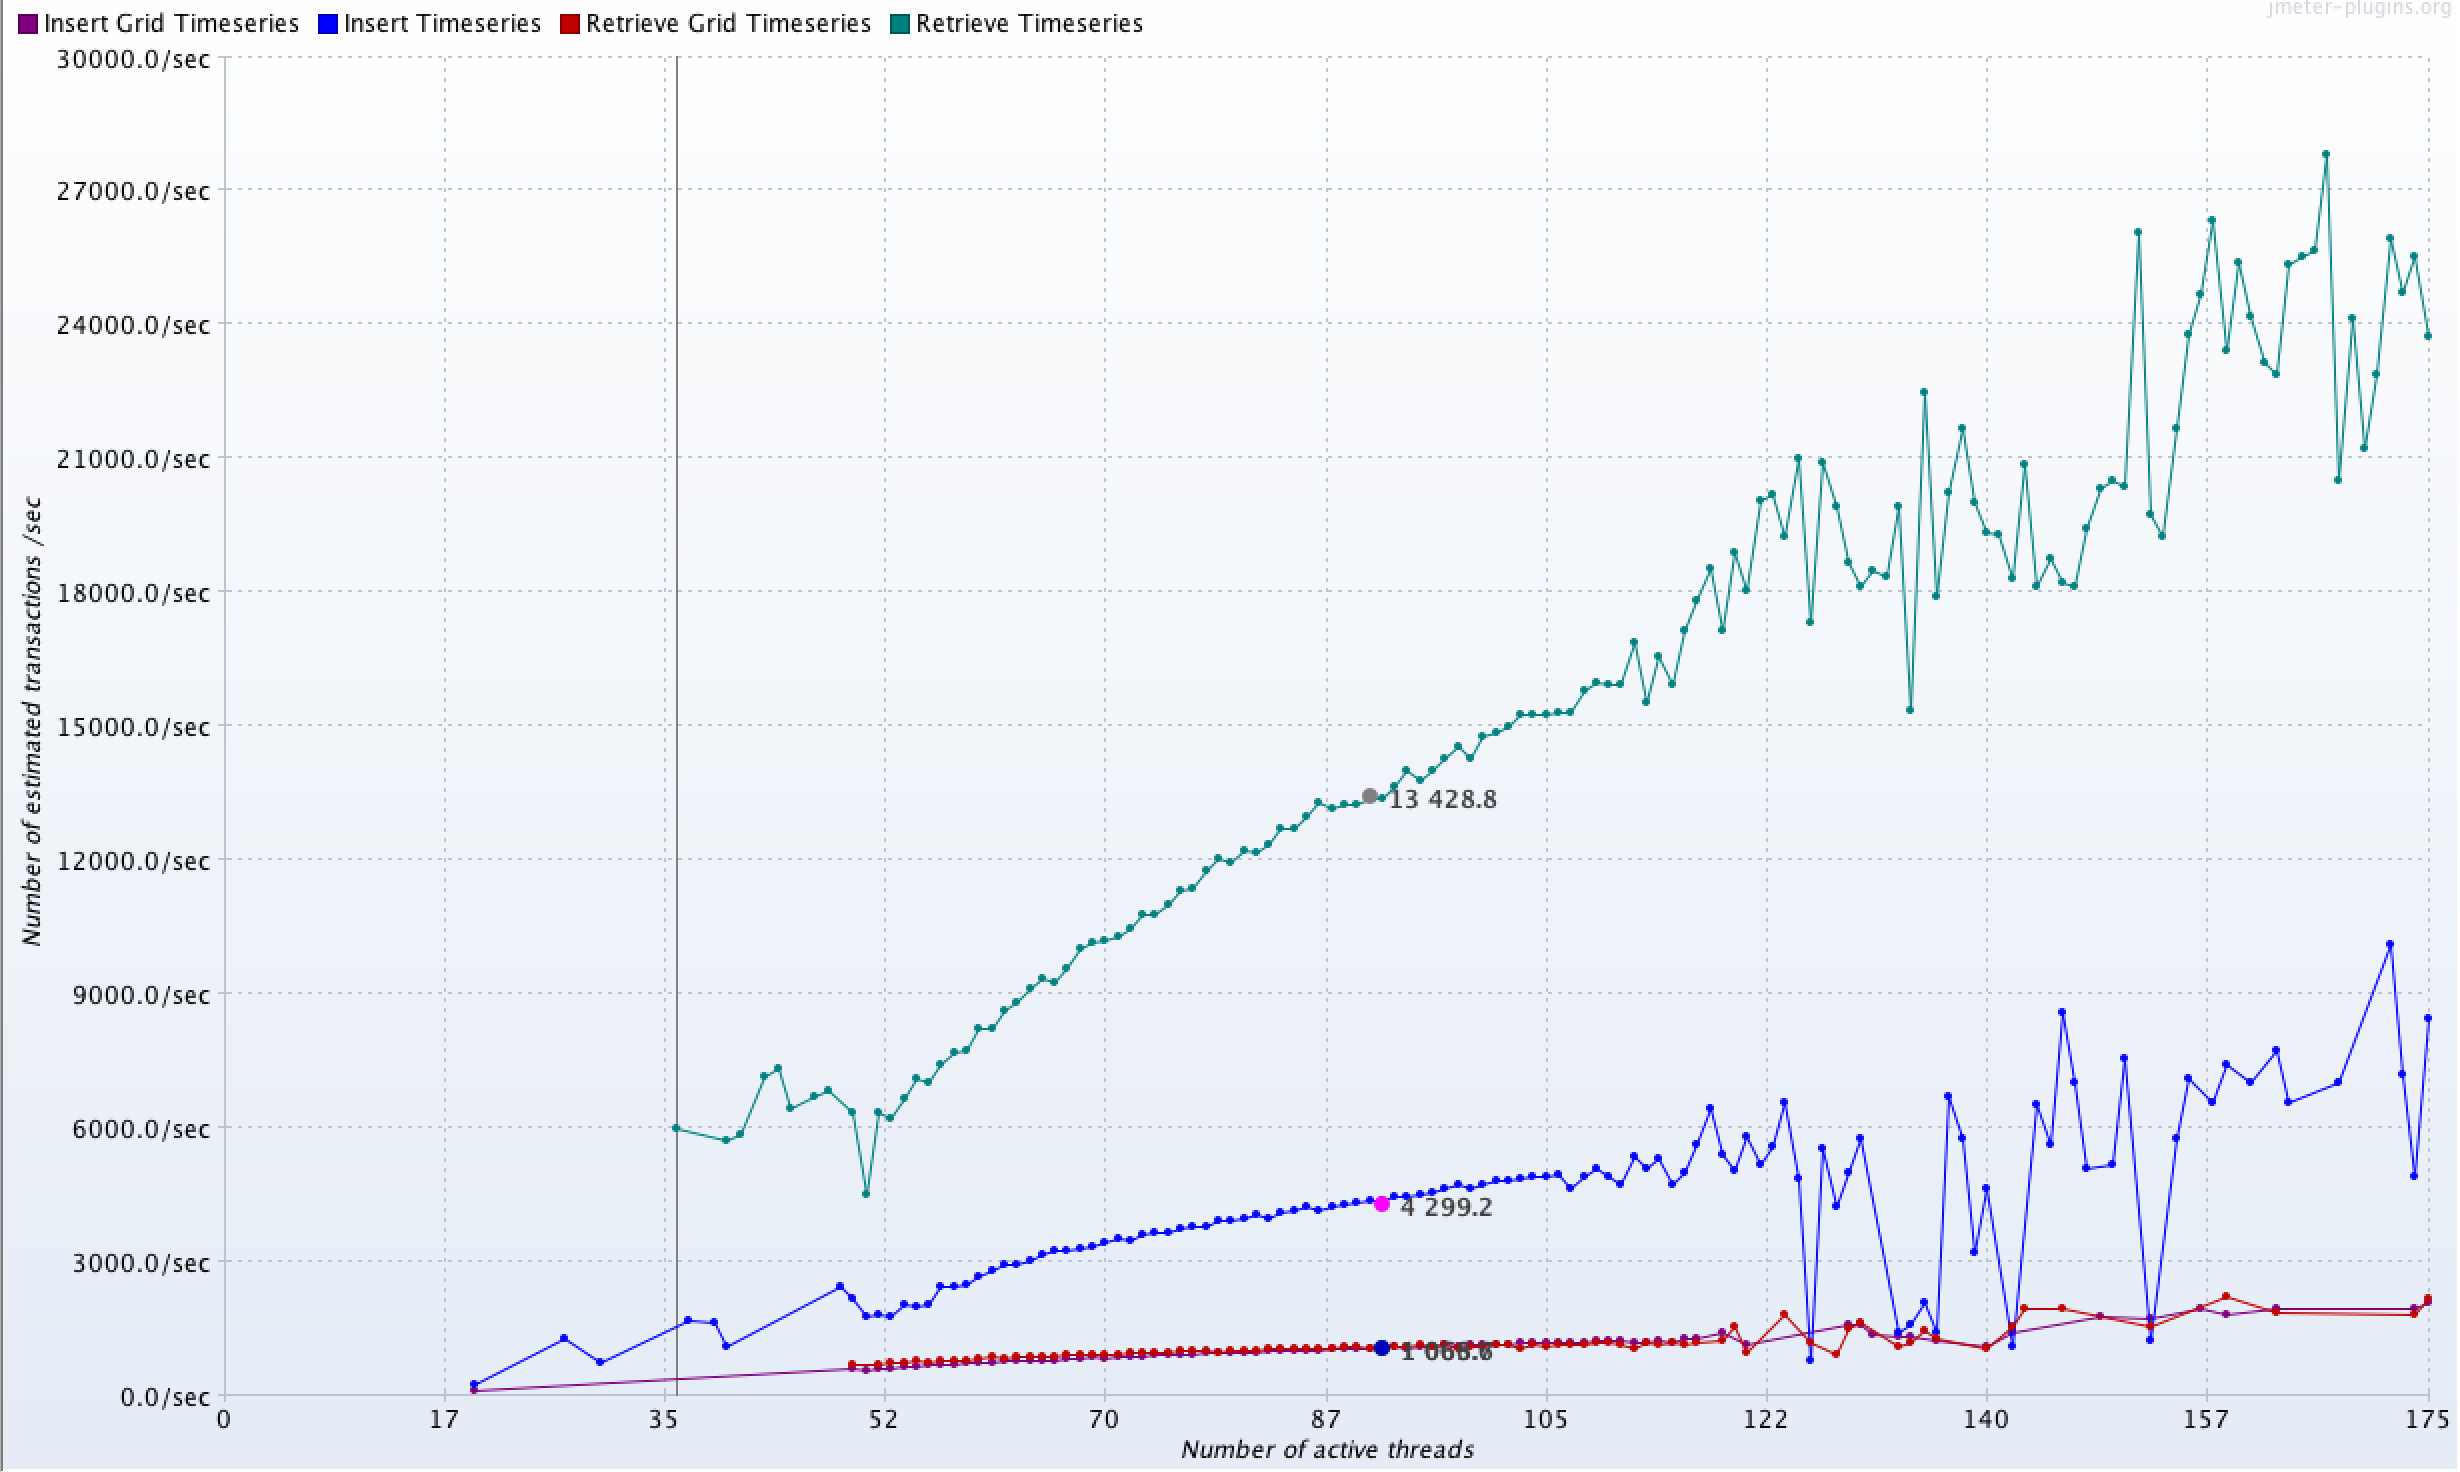
\includegraphics[width=0.5\textwidth]{results/obs/all_auto/obs_all_auto_15m_transaction_throughtput_vs_threads.png}}
%\caption{Transnational throughput vs number of active threads while performance test with 15min data and auto-scaling enabled.}
%\label{pfi:test_obs_auto_all_15_min_throughput_vs_threads}
%\end{figure}

%\cref{pfi:test_obs_auto_all_15_min_throughput_vs_threads} shows the total server's transaction throughput against the number of active threads.
%The formula for total server transaction throughput is \(<active threads> * 1 second / <1 thread response time>\) \cite{JMeterPluginsTransactionPlugin}. It shows the statistical maximum possible number of transactions based on the number of users accessing the application.
%By combining the \cref{pfi:test_obs_auto_all_15_min_latency_vs_hits}, this graph shows that the throughput of the system gets increased without much change in the latency, thus it proves the scalability of the \acrshort{wdias}.
\dbc{I'm removing Fig. 7 as it's a forecast not actual results. Ok to keep this in thesis.}

\begin{figure}[tb!]
    \centering
    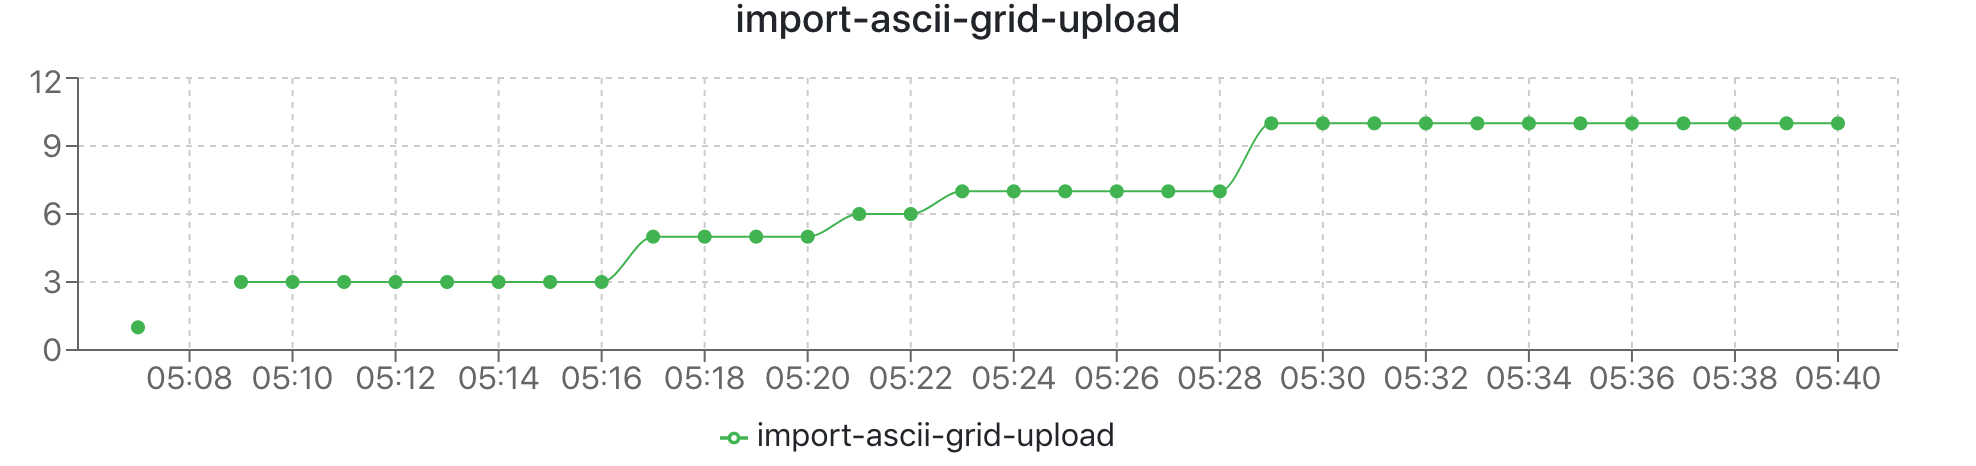
\includegraphics[width=0.5\textwidth]{results/obs/all_auto/obs_all_auto_15m_import_grid_pod.png}
    \caption{Number of running replicas of import ascii grid microservice over time with auto-scaling enabled.}
    \label{pfi:obs_all_auto_15m_import_grid_pod}
\end{figure}

\dbc{x and y axis of \cref{pfi:obs_all_auto_15m_import_grid_pod} need to be labelled}

As the performance bottleneck was mostly on microservices handing grid data, in \cref{pfi:obs_all_auto_15m_import_grid_pod}, we look at how the number of \textit{import-ascii-grid-upload} pods are scheduled with time. \acrshort{k8s} auto-scalar was allowed to scale up to ten pods with a CPU utilization threshold of 80\%. A new pod was allowed to initiate with a single virtual CPU (vCPU) and was able to scale up to two vCPUs per pod. As shown in the graphs, three pods were scheduled initially as per the configuration of the helm chart. As the workload increased, a new pod was spawned when the average CPU utilization reached 80\%. Once the 10 pods were reached no new pods were spawned. Pods were also able to scale vertically up to two vCPUs. From the 0.18\% failed insert grid data operations, most of them were caused once the ten pod and 2 vCPUs per pod limit was reached. It was further noted that once the workload is cut off, the system gradually reduces the number of pods and reach the minimum configure value. 
\dbc{Up to this point we didn't use the word pod. Would it be better to stick to word containers? Also, we never talked about a helm chart.}
\dbc{Either in Sec II.B or III.A we need to briefly mention that grid operations are difficult to handle compared to scalar and vector.}
\dbc{import-ascii-grid-upload was never mentioned}

%%%%%%%%%%%%%%%%%%%%%%%%%%%%%%%%%%%%%%%%%%%%%%%%
\subsection{Performance Metrics Analysis}
\label{psubse:performance_metrics}

%The \emph{Latency} for each operation type kept constant over the whole test plan run time without any significant change. When the request size increased from 24 data points to 96 data points, the latency increase throughout the whole test plan with a smaller number. But for each test run, the latency kept constant over time.
%During the \cref{ptab:obs_all_auto_15_min_summary_throughput} test run, the performance of the Grid data got better when compared to \cref{ptab:obs_all_15_min_summary_throughput}. This means by adding more resources to the \acrshort{wdias}, it can handle more workload on the system.

%While keeping the latency constant without significant change, the \emph{throughput} of the \acrshort{wdias} kept constant while increasing the request size from 60min data (24 data points) to 15min data (96 data points) for all the data types such as Scalar, Vector, and Grid.
%When the number of active threads increased, the \acrshort{wdias} able to provide the same throughput with maintaining the latency stable.

%When looking into the \emph{resource utilization} of \acrshort{wdias}; since it is using the \acrshort{k8s} as the container orchestration system, it allows us to scale up and cool down the system as required based on the workload. This demonstrates the test plan of \cref{ptab:obs_all_15_min_summary_throughput}, and the system gets scale up to the maximum at the peak time. Then cool down to a single pod after finishing the test cases.
%Given above \acrshort{wdias} can run from 1 CPU node to nodes with 100 CPUs. As described in the \cref{pse:wdias_architecture}, it uses many of the concepts of modern microservice architecture to create stateless, failover, redundant microservice to achieve such capabilities.

%The \acrshort{wdias} supports \emph{auto scaling} by out of the box with \acrshort{k8s}. Services can configure with a maximum number of pods to avoid over resource usage. When there is not much workload on the system, the system cools down to fewer pods to save more resources. When there is an issue with a pod, \acrshort{k8s} auto-schedule another pod and remove the unhealthy pod. Also, it allows updating the system without any downtime with rollback updates.

%\emph{Risk of unable to process data} during the test performance, the \acrshort{wdias} processed many requests with higher request size than the normal usage with a lower rate of failures to process the requests, mainly with insert Grid data. If the usage of \acrshort{wdias} wants to reduce the risk of unable to process data, then the system can configure to run with redundant pods to handle spike of workloads. Also while configuring for the auto-scaling, the \acrshort{k8s} can configure to maintain a lower amount of CPU usage such as 50\% to 60\% rather than 80\%. Such configuration with always spawn new pods to handle double of current peak load.

%%%%%%%%%%%%%%%%%%%%%%%%%%%%%%%%%%%%%%%%%%%%%%%%%%%%%%%%%%%%%%%%%%%%%%%%%%%%%%%%
\subsection{Discussion}
\label{psubse:discussion}

As observed from above analysis \acrshort{wdias} could handle increasing workloads (in terms of both the request rate and request size) in a salable manner without a significant increase in latency or errors. It was further noted that auto-scaling containers lead to better performance at a reduced cost. \acrshort{wdias} has several other features/properties that is not covered under above analysis. For example, the extension module enables various prepossessing modules to be integrated into the system as plugins.
With large-scale container orchestration, \acrshort{wdias} can be made to scale from a single vCPU node to nodes with 100s of vCPUs. Moreover, due to the microservices architecture, \acrshort{wdias} can create stateless and redundant modules with failover capabilities. For example, when there is an issue with a pod, container orchestration platform could auto-schedule another pod. Furthermore, microservices allow updating the system without any downtime with rollback updates.
\dbc{Is ``rollback updates'' a standard word?}
\dbc{While performance testing didn't we run in preprocessing modules? If so, it need to be clearly mentioned}

Somewhat high variability in insert and retrieval operations was due to the use of a single instance of InfluxDB to handle scalar and vector data. While the use of a single instance to avoided potential data consistency issues, it also constrained the throughput and increased the latency. Due to the microservices architecture it is possible to easily extend \acrshort{wdias} to support timeseries databases with sharding and replication features (e.g.,InfluxDB Enterprise edition). Further the use of flat files for netCDF affected the performance of grid data related requests. As microservices can be written in any programming language, more computationally heavy modules such as \acrshort{netCDF}-based grid data processing functions could be written in C or FORTRAN as opposed to our Python wrapper. 
\dbc{one InfluxDB for both or one each?}

%Also, \acrshort{wdias} provides a more generic open interface approach to create more preprocessing modules. Since \acrshort{wdias} is an open-source system, it expects more modules to be created by the community. When compared to other systems like \acrshort{fews}, the current system only have few extensions but it is more easy to add new extensions compared to other systems.


%%%%%%%%%%%%%%%%%%%%%%%%%%%%%%%%%%%%%%%%%%%%%%%%%%%%%%%%%%%%%%%%%%%%%%%%%%%%%%%%
\section{Summary}
\label{pse:summary}

We presented a weather data integration and assimilation system based on the microservices architecture and container orchestration. As demonstrated by the performance analysis, \acrshort{wdias} can ingest, transform, and export scalar, vector, and grid timeseries data in multiple formats with good throughput and latency characteristics. Moreover, the combination of microservice architecture and container orchestration results in a extensible, scalable, available, and resource efficient system. In addition to adding more extension modules to manipulate timeseries data, in future, we plan to extend \acrshort{wdias} by introducing publisher-subscriber capabilities for data dissemination and support irregular grid and polygon data. Further, \acrshort{wdias} could be packaged as an infrastructure as code, using a tool like Terraform, to simplify the deployment on any Cloud provider. 



%%%%%%%%%%%%%%%%%%%%%%%%%%%%%%%%%%%%%%%%%%%%%%%%%%%%%%%%%%%%%%%%%%%%%%%%%%%%%%%%
\section*{Acknowledgment}
\label{pse:ack}
This research is supported in part by the grant from the Center for Urban Water, Sri Lanka.

%%%%%%%%%%%%%%%%%%%%%%%%%%%%%%%%%%%%%%%%%%%%%%%%%%%%%%%%%%%%%%%%%%%%%%%%%
\graphicspath{ {./images/} }
\newacronym{wdias}{WDIAS}{Weather Data Integration and Assimilation System}

\newacronym{fews}{Delft-FEWS} {Deltares FEWS}
\newacronym{lead}{LEAD}{Linked Environments for Atmospheric Discovery}
\newacronym{dias}{DIAS}{Data Integration and Assimilation System}
\newacronym{madis}{MADIS}{Meteorological Assimilation Data Ingest System}

\newacronym{nwm}{NWMs}{Numerical Weather Models}
\newacronym{soa}{SOA}{Service Oriented Architecture}
\newacronym{wrf}{WRF}{Weather Research and Forecast}
\newacronym{esb}{ESB}{Enterprise Service Bus}
\newacronym{microservice}{Microservice}{Microservice Architecture}

\newacronym{netCDF}{netCDF}{Network Common Data Form}
\newacronym{GRIB}{GRIB}{General Regularly-distributed Information in Binary form}
\newacronym{csv}{CSV}{Comma-separated Values}

\newacronym{rdbms}{RDBMS}{Relational Database Management System}
\newacronym{k8s}{K8s}{Kubernetes}
\newacronym{eks}{Amazon EKS}{Amazon Elastic Kubernetes Service}

\newacronym{go}{Go Lang}{Go Programming Language}
\newacronym{rps}{RPS}{Requests Per Second}
\newacronym{api}{API}{Application Programming Interface}
\newacronym{rps}{RPS}{Request per Second}

\newacronym{curw}{CUrW-SL}{Center for Urban Water, Sri Lanka}

% \printbibliography[title={References}]
\bibliographystyle{IEEEtran}
\bibliography{mendeley}

\dbc{Still these references are not quite IEEE style. I fixed some of the references in your bib file. Also, I have had issues with IEEE template in Overleaf.}
\gkc{It is same as the class mentioned here: https://www.ieee.org/conferences/publishing/templates.html. I think, we have to add correct data in the bib to get it working. Previously, some reference showed with Capitals due to mendeley add the text as Capital rather Title case.}

\end{document}
